\documentclass{article}
\usepackage[francais]{babel}
\usepackage[utf8]{inputenc}  
\usepackage{listings}
\usepackage{graphicx}
\usepackage{color}
\usepackage{float}

% Style for c code
\definecolor{mygreen}{rgb}{0,0.6,0}
\definecolor{gray}{rgb}{0.5,0.5,0.5}
\definecolor{mymauve}{rgb}{0.58,0,0.82}
\definecolor{backcolour}{rgb}{0.95,0.95,0.92}

\lstdefinestyle{cstyle}{ 
  language=C,
  backgroundcolor=\color{backcolour},   
  basicstyle=\footnotesize,        % the size of the fonts that are used for the code
  captionpos=b,                    % sets the caption-position to bottom
  commentstyle=\color{mygreen},    % comment style
  deletekeywords={...},            % if you want to delete keywords from the given language
  escapeinside={\%*}{*)},          % if you want to add LaTeX within your code
  keepspaces=true,                
  keywordstyle=\color{blue},       % keyword style
  otherkeywords={*,...},           % if you want to add more keywords to the set
  numbers=left,                   
  numbersep=5pt,                   % how far the line-numbers are from the code
  numberstyle=\tiny\color{gray}, % the style that is used for the line-numbers
  rulecolor=\color{black},        
  showspaces=false,               
  showstringspaces=false,          % underline spaces within strings only
  showtabs=false,                  % show tabs within strings adding particular underscores
  stepnumber=1,                    % the step between two line-numbers. If it's 1, each line will be numbered
  stringstyle=\color{mymauve},     % string literal style
  tabsize=2,	                   % sets default tabsize to 2 spaces
  title=\lstname                   % show the filename of files included with \lstinputlisting; also try caption instead of title
}

\lstset{style=cstyle}

\title{Simulation de la gravitation universelle}
\author{Benjamin \bsc{Angelaud} - Adrien \bsc{Guilbaud}}
\begin{document}
\maketitle
% gregoire.pichon@inria.fr
% Deadline 5 novembre, minuit

% n particules plan 2D
% mémoire limitée par processus

% *une masse mi
% *une position vec(pt(Mi)) 
% *une vitesse vec(vt(Mi))

% \paragraph{}
% $ F_t(M_i, M_j) = F_t(M_j, M_i) * \overrightarrow{u}_{ij} $
% \paragraph{}
% $ F_t(M_i, M_j) = G \frac{m_i m_j}{(M_i M_j)^2} * \overrightarrow{u}_{ij} $
% \paragraph{}
% uij unitaire dirigé de Mi à Mj
% \paragraph{}
% $ F_t(M_i) = \sum_{i=1}^{n}  F_t(M_i, M_j) i \not= j $
% \paragraph{}
% $ \overrightarrow{a_t(M_i)} = \frac{F_t(M_i)}{m_i} $
% \paragraph{}
% Discrétitation avec un pas de temps dt: 
% $ \overrightarrow{pt+dt}(M_i) = \overrightarrow{pt}(M_i) + \overrightarrow{vt}(M_i)dt + \frac{\overrightarrow{at}(M_i)}{2} * dt^2 $
% \paragraph{}
% v(t)+dt(Mi)  =vt(Mi) + at(Mi)dt
% \paragraph{}
% Il faut fixer un dt: petit si les particules sont proches pour éviter les colissions.


\section{Version séquentielle}
Avant de commencer la version parallèle, nous avons d'abord choisi de programmer en séquentiel dans le but de pouvoir valider notre code sans que les erreurs pouvant être provoqué par MPI ne rentre en ligne de compte. De plus, le code permettant le calcul des forces pouvait être entierement réutilisé dans la version parallèle. Cela nous permet également d'avoir un bon point de comparaison pour comparer les résultats en obtenus en MPI.

\subsection{L'implémentation séquentielle}
Nous avons créé une structure permettant de stocker l'état des particules (i.e. la masse, un vecteur position et un vecteur vitesse). En effet, il n'est pas nécessaire de stocker l'accéleration directement dans la structure car elle est recalculée à chaque pas de temps.

\begin{figure}[h]
  \centering
  \begin{lstlisting}[language=C]
    typedef struct particle_s{
      double m;
      double p[2];
      double v[2];
    }particle_t;\end{lstlisting}
  \caption{Structure d'une particule}
\end{figure}

Nous avons plutôt choisi un type de donnée AoS que SoA.
La fonction permettant de calculer les intéractions entre particules consiste en 2 boucles imbriquées parcourant chacune un ensemble de particules. Pour calculer ces intéractions, nous avons besoins de la masse et de la position des particules. Si nous utilisons un type SoA, avec un grand nombre de particules, une partie du tableau contenant les masses sera chargé dans le cache, puis une partie du tableau des positions. Le cache alternera donc une ligne contenant les masses et une ligne contenant les positions. Cependant, il faut les positions de 2 particules pour calculer la distance les séparant. Dans 
un seul des tableaux de masses ou de positions pouraient rester dans le cache, provoquant un cach miss dés que nous aurions besoin d'une donée présente dans l'autre tableau. 
Avec un type AoS les données relatives aux particules sont stockées de façon contigüe en mémoire et toutes les données chargées dans le cache sont utilisées ce qui réduit le nombre de cach miss.


\begin{figure}[h]
  \centering
  \includegraphics[scale=0.5]{Diagramme1.jpeg}
  \caption{\label{fig:label} }
\end{figure}
A partir de point la, il y aura des cache miss à chaque nouvelle ligne de cache. Les positions vont donc être écrites par dessus les masses ce qui produira encore des cach miss.

\subsection{Exécution séquentielle}

\begin{figure}[h]
  \centering
  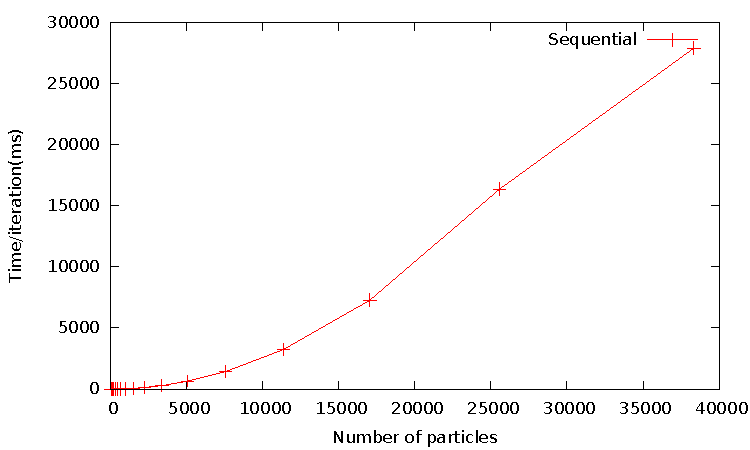
\includegraphics[scale=0.7]{ResultTDP2/seq_temps_iter/seq.pdf}
  \caption{\label{seq_ti}Temps/itération en fonction du nombre de particules}
  
\end{figure}
Nous pouvons observer sur cette courbe que le temps d'une itération est fortement dépendant du nombre de particules. En effet, l'algorithme utilisé est en $ O(n^2) $ car chaque particule doit intéragir avec les $ n-1 $ autres particules.


\section{Version MPI}
\subsection{Choix des communications}
Nous nous sommes ici intéressé aux différents modes de communications disponibles avec MPI dans le but de comparer leurs impacts sur les performances de l'application. Dans un premier temps, nous avons utilisé les comunications point-à-point non-bloquantes. Cependant, les communications étant toujours appelées avec les mêmes arguments, il était possible de les transformer en communications persistantes.

\begin{figure}[h]
  \centering
  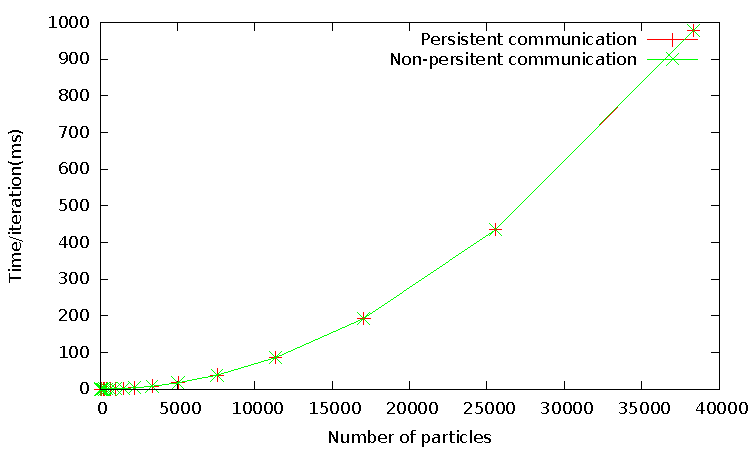
\includegraphics[scale=0.5]{ResultTDP2/mpi_comm/mpi_comm_singlenode.pdf}
  \caption{\label{fig:tf(n)1}Comparaison du type de communications sur 1 noeud}
\end{figure}

\begin{figure}[h]
  \centering
  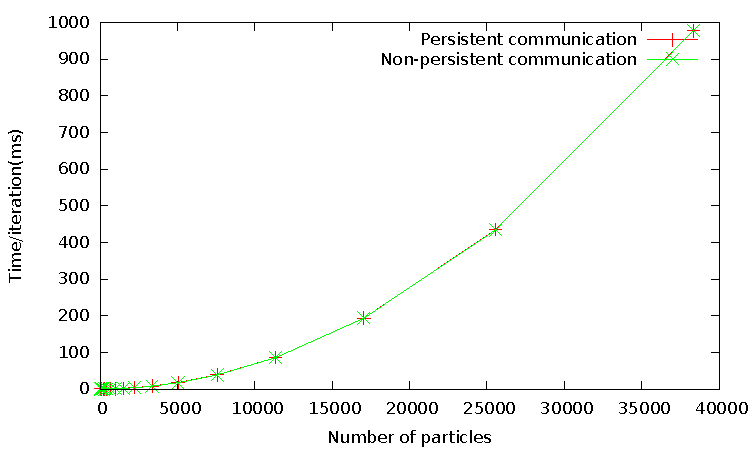
\includegraphics[scale=0.5]{ResultTDP2/mpi_comm/mpi_comm_multinode.pdf}
  \caption{\label{fig:tf(n)2}Comparaison du type de communications sur 2 noeuds}
\end{figure}


\paragraph{}
Commentaires sur les courbes

\subsection{Structure de données MPI}
Nous avons ensuite voulu comparer l'impact de la taille de la structure de données que les processus s'échangaient. Pour cela, nous avons d'abord créé un datatype MPI grace à la fonction MPI\_Type\_create\_struct contenant les mêmes données que la structure classique. Nous avons ensuite comparé les temps d'éxécution avec ce type de données et un second ne contenant pas les vitesses.

\begin{figure}[!h]
  \centering
  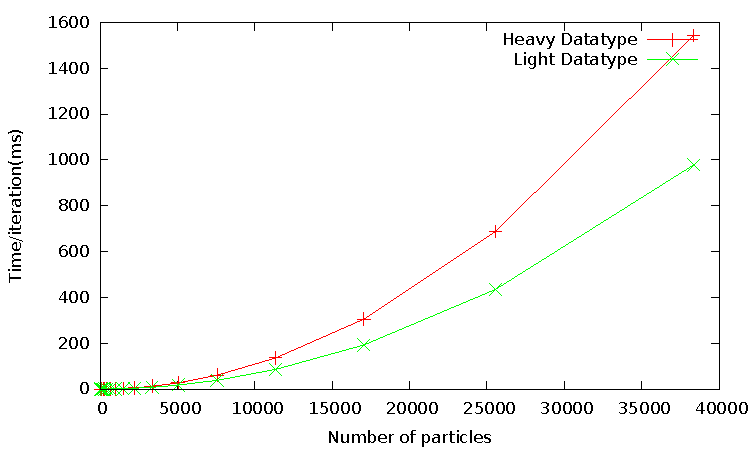
\includegraphics[scale=0.5]{ResultTDP2/mpi_datatype/mpi_datatype_singlenode.pdf}
  \caption{\label{fig:tf(n)data1}Comparaison du datatype sur 1 noeud}
\end{figure}

\begin{figure}[!h]
  \centering
  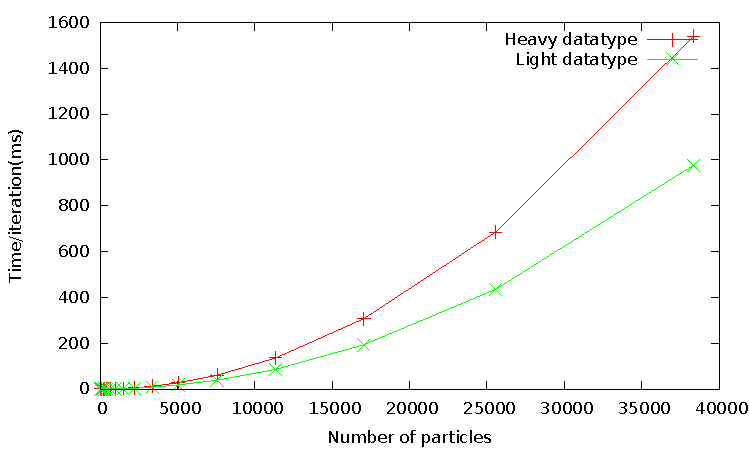
\includegraphics[scale=0.5]{ResultTDP2/mpi_datatype/mpi_datatype_multinode.pdf}
  \caption{\label{fig:tf(n)data2}Comparaison du datatype sur 2 noeuds}
\end{figure}


\paragraph{}
Sur la figure \ref{fig:tf(n)data1}, nous pouvons observer que la durée d'une itération est bien moindre lorsque l'on n'envoie plus les vitesses des particules lors des transmissions. Pour chaque itérations de la simulation, $ nbProc \times (nbProc - 1) $ messages sont envoyés. Nous économisons donc l'envoi de $ nbMessages \times nbIter \times \frac{nbParticules}{nbProc} \times 2 $ double par rapport à l'autre type de donnée. Pour 10000 particules et 1000 itérations sur 20 processus, cela représente 2,8 Go de données non-envoyées.


\section{Comparaison}
\subsection{Procédure de test}
Pour réaliser l'ensemble des courbes présentées, nous avons utilisé la même procédure. Que ce soit dans la version séquentielle ou la version paralléle, nous mesurons seuleument le temps pris pour calculer l'ensemble des intéractions puis la mise à jour des positions et vitesses. En MPI, ce temps prend en compte le temps des communications.


\section{Améliorations possibles}
\subsection{Algorithmique}
Afin d'améliorer les performances de cette application, nous pourions éviter de calculer les interactions entre toutes les particules. En effet, la force gravitationnelle étant inversement proportionnelle à la distance au carré, elle devient négligeable pour des particules trés éloignées. Au lieu de découper l'espace de manière had-oc, nous pourrions le diviser en une grille. Chaque bloc ainsi obtenu ne devrait intéragir qu'avec lui même et les 8 blocs adjacents. Ceci réduirait le temps de calculs des intéractions ainsi que la quantité de données échangée par les processus MPI.

\paragraph{} 
Il faut par contre pouvoir déterminer la taille de ces blocs afin de ne pas complétement fausser les résultats.

\begin{figure}[ht]
  \centering
  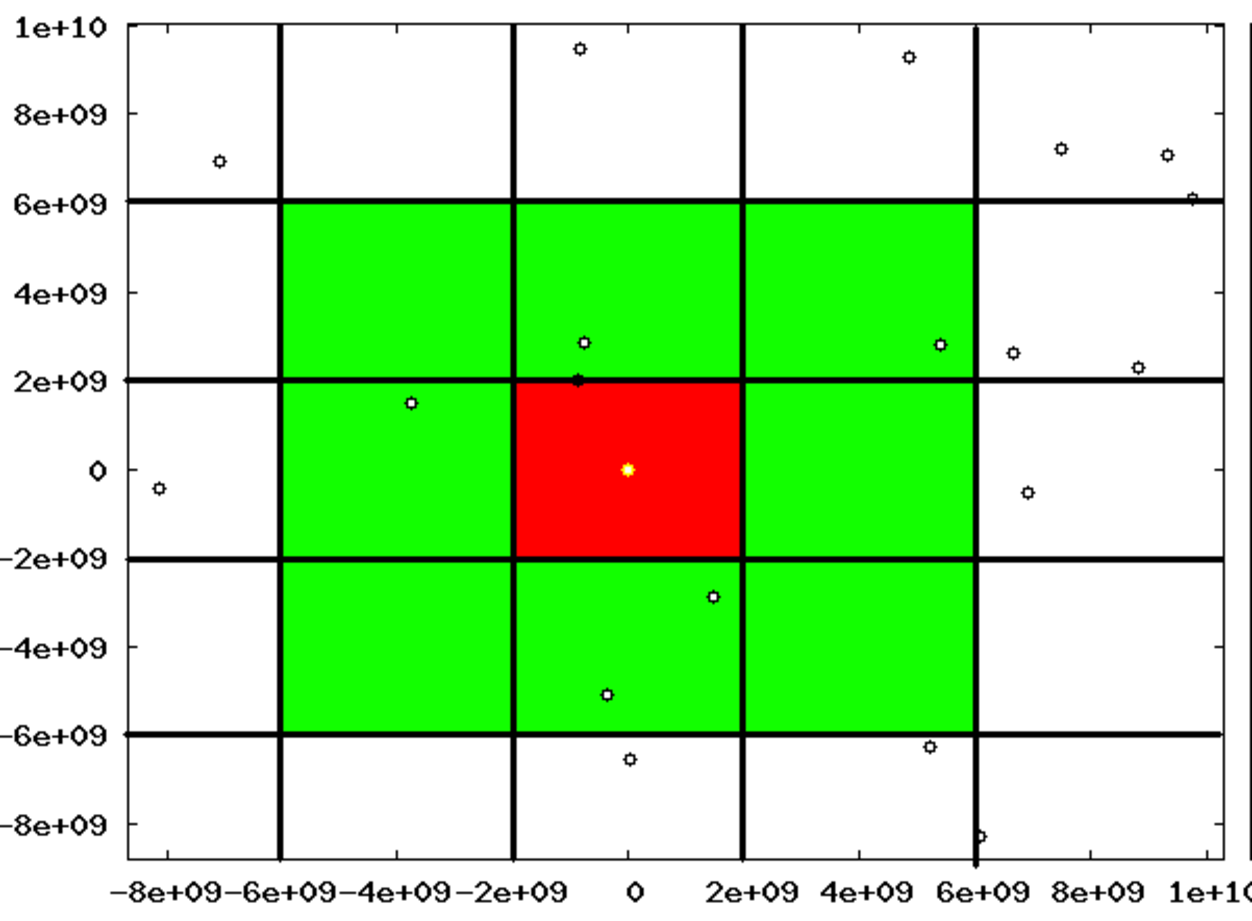
\includegraphics[scale=0.5]{algobloc.pdf}
  \caption{\label{fig:label} }
\end{figure}


\end{document}
